\chapter{Theory}

Two of the studies presented within this thesis are for prospective measurements looking at the $H\rightarrow WW$ branching ratio and the forward-backward asymmetry in \ttbar~ production at CLIC during the 1.4~TeV stage. As such it is important to first examine the significance of these measurements in the context of the physics programme of CLIC and the wider state of particle physics.


\section{The Standard Model}

\begin{figure}
  \centering
  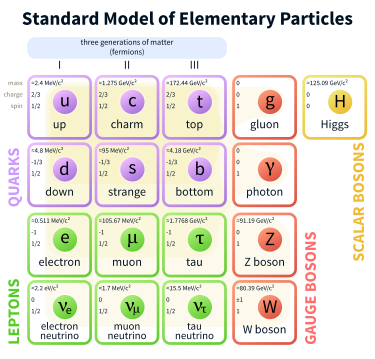
\includegraphics[width=0.55\textwidth,keepaspectratio]{Theory/fig/smparticles.png}
  \caption[Particles of the Standard Model]{Particles of the Standard Model}
  \label{fig:smparticles}
\end{figure}

The \ac{SM} is an effective quantum field theory representing our best current description for describing fundamental particles and the interactions between them. It consists of twelve spin-$\frac{1}{2}$ fermions (and their corresponding antiparticles), four spin 1 gauge bosons and one spin 0 scalar boson as shown in \reffig{fig:smparticles}. The interactions of the model are described by an $SU(3)_{C}\oplus SU(2)_{L}\oplus SU(1)_{Y}$ local gauge symmetry in which the SU(3) symmetry components represent transformations effecting colour charge (\ac{QCD} interactions) while the $SU(2)\oplus SU(1)$ symmetry describes interactions involving weak isospin, and weak hypercharge (\ac{QED} interactions) that leave the lagragian of the system invariant. The symmetries of these groups and the quantum fields associated with them can be used to describe the three mechanisms through which fermions interact- the strong, weak and electroweak forces. No explanation of gravitational interactions is currently provided by the \ac{SM}. 


Within the model the fermions can be split into two categories depending on the ways they can interact. The first category are leptons which possess weak hypercharge but no colour and so can interact through the weak force but not the strong. They consist of the electron(e), muon($\mu$), tau($\tau$), electron neutrino($\nu_{e}$), muon neutrino($\nu_{\mu}$) and tau neutrino($\nu_{tau}$). The electron, muon and tau also possess charge allowing them to interact through the electromagnetic force. The second category are quarks which all possess charge, hypercharge and colour allowing them to interact via all three forces. The quark family consists of the up(u), down(d), charm(c), strange(s), top(t) and bottom(b) quarks. The three forces are mediated by the gauge bosons. The electromagnetic and strong forces are mediated by the photon and gluon respectively, both of which are massless particles giving them infinite range. (In practice this isn't quite true for the gluon as the fact it carries colour charge results in a powerful attraction between itself and the particle emitting and so the gluon becomes confined to short range interactions.) The weak force is mediated by three separate particles- the Z, W$^+$ and W$^-$- all of which are massive, limiting their range. 



\section{Higgs Physics and the Origin of Mass}

Without the presence of the Higgs Boson, the standard model predicts that all fermions and bosons should be massless. Brout, Englert and Higgs (REFERENCE) proposed that mass terms could be generated within the \ac{SM} via the addition of a complex, scalar doublet of the group $SU(2)_{L}$:


\begin{align}
\phi = \begin{pmatrix} \phi^{+} \\ \phi^{0} \end{pmatrix} 
\end{align}



\section{Higgs Measurements at CLIC}
\begin{figure}
  \centering
  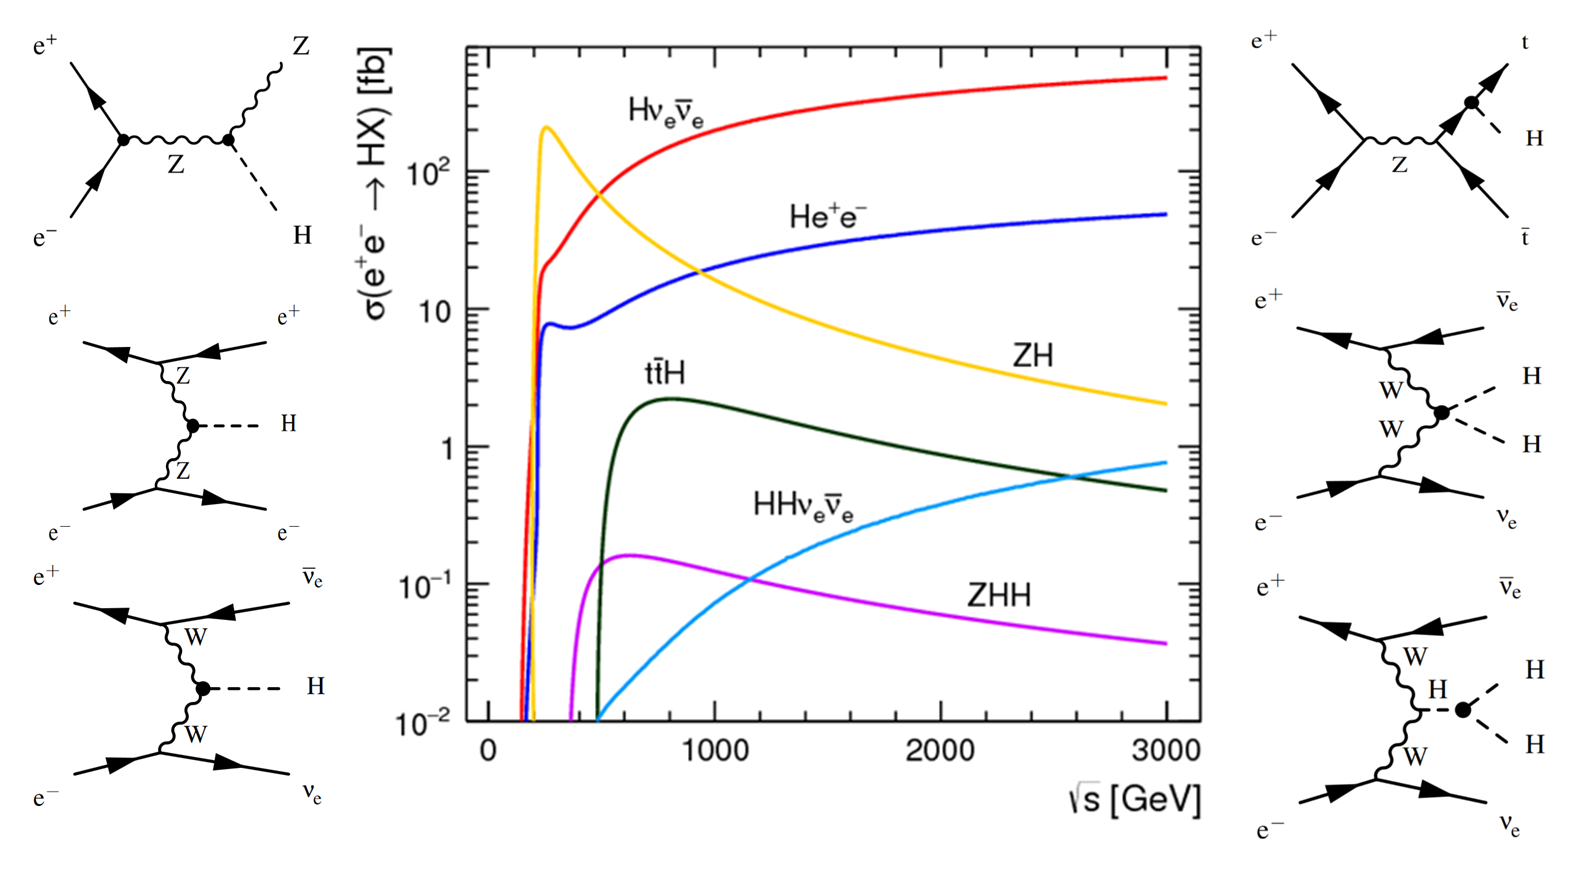
\includegraphics[width=0.95\textwidth,keepaspectratio]{Theory/fig/HiggsProcessesExtra.png}
  \caption[Cross Sections For Higgs Production Mechanisms]{Cross Sections For Higgs Production Mechanisms}
  \label{fig:higgsXSecs}
\end{figure}

The CLIC physics programme has a large focus on characterising the Higgs boson due to the large uncertainties on many of it's associated properties relative to other sectors of the standard model. In particluar it will aim to measure the mass, width, spin and couplings of the Higgs in a model independent manner. Electron positron collisions provide access to numerous Higgs production mechanisms which can be seen in \ref{fig:higgsXSecs}. Due to the strong energy dependence on many of the cross sections on energy, different processes will be of interest at each of the three energy stages operated at CLIC. At 380GeV the focus will predominantly be on measuring the Higgsstrahlung ($ZH$) process, while at higher energies vector boson fusion ($H\nu\nu,Hee$) dominates and new processes such as di-Higgs production become accessible. A summary of all the results from current Higgs studies performed by CLIC is available in \cite{Abramowicz:2016zbo}.

\subsection{Higgsstrahlung}

\begin{figure}
  \centering
  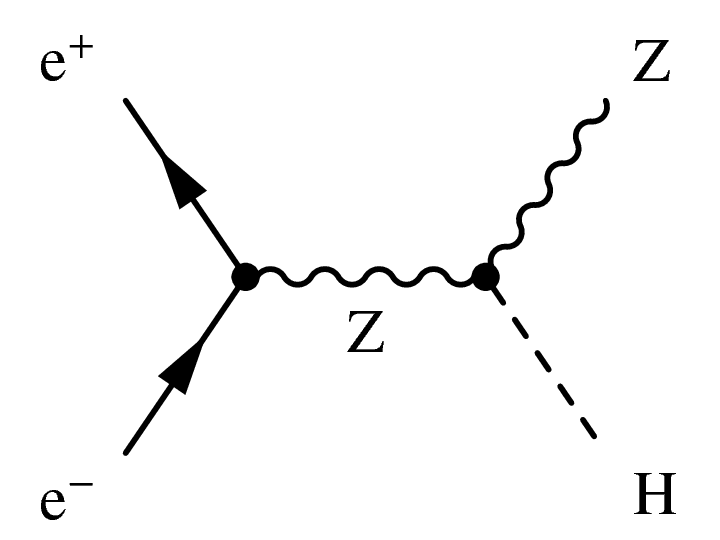
\includegraphics[width=0.45\textwidth,keepaspectratio]{Theory/fig/HiggsStrahlung.png}
  \caption[The Higgstrahlung Process]{The Higgstrahlung Process}
  \label{fig:higgsstrahlung}
\end{figure}


One of the key aims of the experiment will be to examine the Higgsstrahlung process shown in \ref{fig:higgsstrahlung}. In this process, if the four momentum of the Z boson can be measured to high precision, then because the initial conditions of the collision are well known, one can determine the mass of the particle it is recoling against ($m_{rec}^{2} = s + m_{z}^{2} - 2E_{z}^{2}$) and infer the presence of the Higgs. This allows properties such as the Higgs mass, cross-section and coupling to the Z to be measured without actually ever measuring the decay products of the Higgs boson which in turn allows the measurements to be model independent as few assumptions must be made about the interactions of the Higgs. This method is not possible at hadron colliders such as the LHC where, even though the Higgsstrahlung process still occurs, as the four momentum of the colliding particles can never be known to as high a level of precision due to their composite nature. Using the clean signal from cases where the Z decays to a pair of muons or electrons it is possible to measure the recoil mass to high precision and thus determine the mass of the Higgs to $\Delta m_{H} = 110~MeV$ (see figure \ref{fig:higgsmass} using data from the low energy stage only. This value can be further improved to $\Delta m_{H} = 44~MeV$ when including direction measurement results from the $ee\rightarrow H\nu\bar{\nu}, H\rightarrow b\bar{b}$ channel at 3~TeV. Despite giving a poorer resolution on the Z four momentum, the $Z\rightarrow qq$ higgsstrahlung channel is also considered due to it's larger cross section. Using this channel a limit of $BR(H\rightarrow invis.) <0.97\%$ at 90\% C.L. can be set. 

\begin{figure}
  \centering
  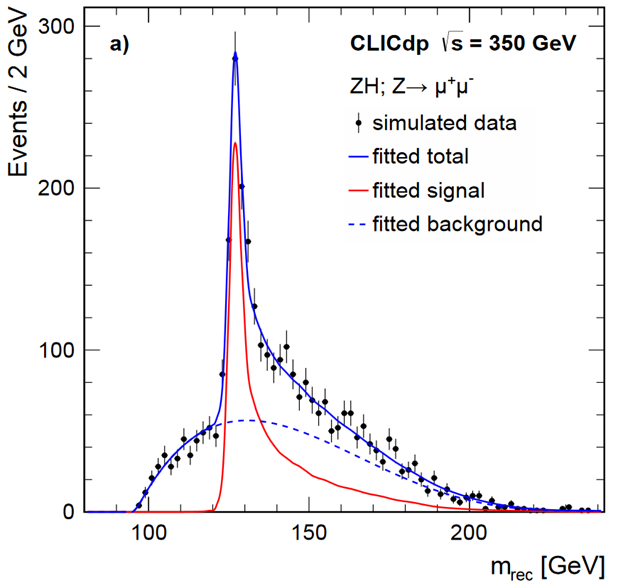
\includegraphics[width=0.45\textwidth,keepaspectratio]{Theory/fig/HiggsRecoilMass.png}
  \caption[Reconstructed recoil mass from Higgsstralung process]{Reconstructed recoil mass from Higgsstralung process}
  \label{fig:higgsstrahlung}
\end{figure}

 
\subsection{Model Independent Extraction of Higgs Couplings}


While the Higgsstrahlung alone allows the mass and branching ratios of the Higgs to be determined, by measuring the rates of several different Higgs processes and combining them in the right ratio, it is further possible to extract the absolute width of the Higgs. One such ``recipe'' proposed for doing this is shown in \ref{modelindependentformula} \cite{Durig:2014lfa}:


\begin{equation}
  \label{modelindependentformula}
  \Gamma_H = \frac{Y_1^2Y_3^2}{Y_4^2Y_2}
\end{equation}

where

\begin{equation}
X_1=\sigma_{ZH} \propto g_{HZZ}^2
\end{equation}

\begin{equation}
  \label{X2}
  X_2=\sigma_{H\nu\bar{\nu}} \times BR(H\rightarrow WW^*) \propto \frac{g_{HWW}^4}{\Gamma_H}
\end{equation}

\begin{equation}
X_3=\sigma_{H\nu\bar{\nu}} \times BR(H\rightarrow b\bar{b}) \propto \frac{g_{HWW}^{2}g_{Hbb}^2}{\Gamma_H}
\end{equation}

\begin{equation}
X_4=\sigma_{ZH} \times BR(H\rightarrow b\bar{b}) \propto \frac{g_{HZZ}^{2}g_{Hbb}^2}{\Gamma_H}
\end{equation}


Currently at the LHC the standard process for extracting couplings from the equivalent measurements of $X_{2,3\&4}$ is to multiply through by the standard model value of the Higgs width. This type of measurement is referred to as `model-dependent` as the values determined for the Higgs couplings carry the implicit assumption that the standard model is correct in it's prediction of the Higgs width. At CLIC, because the width can be measured experimentally there is no need to make this assumption and so the couplings are measured in a ``model-independent'' way. The unique ability of linear colliders to perform model-independent measurements is one of the largest driving factors for constructing and using them as a so called ``Higgs-Factory''. One limiting factor for the model-independent measurements of the couplings is that they are always ultimately dependent on the precision to which the ZH cross section can be measured (predicted to be $\Delta h_{HZZ} = 0.8\%$) as this quantity is always needed in the ratio used to extract $\Gamma_H$. With the exception of $X_1$, the choice of variables used is not unique (e.g. one could replace the production mechanism in $X_1$ and $X_2$ with ZZ-fusion rather than WW-fusion,) however the combination shown here is expected to give the highest precision on $\Gamma_H$ due to the large cross-section associated with WW-fusion and the high branching ratio of $H\rightarrow b\bar{b}$ ($\sim$ 65\%). In chapter \ref{Higgs Analysis} we will present our research on the precision to which $X_2$ from eq \ref{X2} can be measured during the 1.4~TeV run at CLIC.

In practice it is expected that an 11 parameter global fit to multiple variations of these measurements will be performed at each stage of operation to extract the Higgs width and it's couplings to both fermions and bosons. The relevant inputs for these fits are shown in tables (INSERT table 28 and 29 from higgs paper) while the results of the fits are shown in (table 26 and fig 28 from higgs paper.)

For context it is also important to compare these results to what can be expected from current leading experiments such as ATLAS and CMS at the LHC and the predicted precision they will have optained by the time CLIC would begin operation. Because the Higgs width can not be explicitly calculated at Hadron colliders, it is best to compare the model dependent version of the CLIC analysis with those predicted by ATLAS and CMS. In this situation, becuase the precision of the couplings is no longer limited by the precision on $g_{HZZ}$ the predicted precision for CLIC is seen to improve considerably. One can see from figure (SHOW CLIC MODEL DEPENDENT PLOT AND LHC PREDICTIONS) that in almost all cases CLIC is expected to provide a considerable improvement over what can be achieved at the LHC with many of the key parameters associated with the Higgs being measured to sub percent precision.

Ultimately the aim of performing precision measurements is to be allow the validation or rejection of theoretical models. While the results seen so far at the LHC suggest that the observed Higgs Boson is that of the \ac{SM}, their are numerous alternative theories that predict a Higgs like particle with properties similar to what has been observed but which differ to a degree not yet measureable by current experiments. The details of these theories will not be expanded upon within this thesis, however the deviations expected in the Higgs couplings of these theories relative to the \ac{SM} are shown in table (INSERT SNOWMASS TABLE.) These values should only be taken as a rough guideline for the precision required to discover/reject the theories as they are based on the assumption that new physics occurs at a specific scale (in this case 1~TeV,) however it is clear that the level of precision required to provide sensitivity to these models will be greater than what will be possible with the LHC but could be within the scope of the proposed CLIC physics programme.  


\section{Top Quark Physics}

Highest mass in the standard model, not precisely measured, possible sensitivity to BSM physics.

CLIC has a rich program of top physics thanks to it's operation at 380~GeV close to the top pair production threshold.

Beyond the mass and width of the top, one of the key aims will be to measure the coupling of of the top to z/gamma. Provides access to form factors that are sensitive to BSM effects.

Several measurements necessary such as the AFB and cross section

Define what the forward backward asymmetry is, brief history of measurements elsewhere

How it fits in with the calculation of the EW couplings

New physics that can effect these couplings e.g. Z'

